\section{The PRIAM methodology}
In this section we aim to introduce how the PRIAM methodology works on a high
level. In order to achieve this we will first provide a bird's-eye view of the
steps involved and then briefly explain what each step entails.

\begin{figure}[h!]
  \centering
  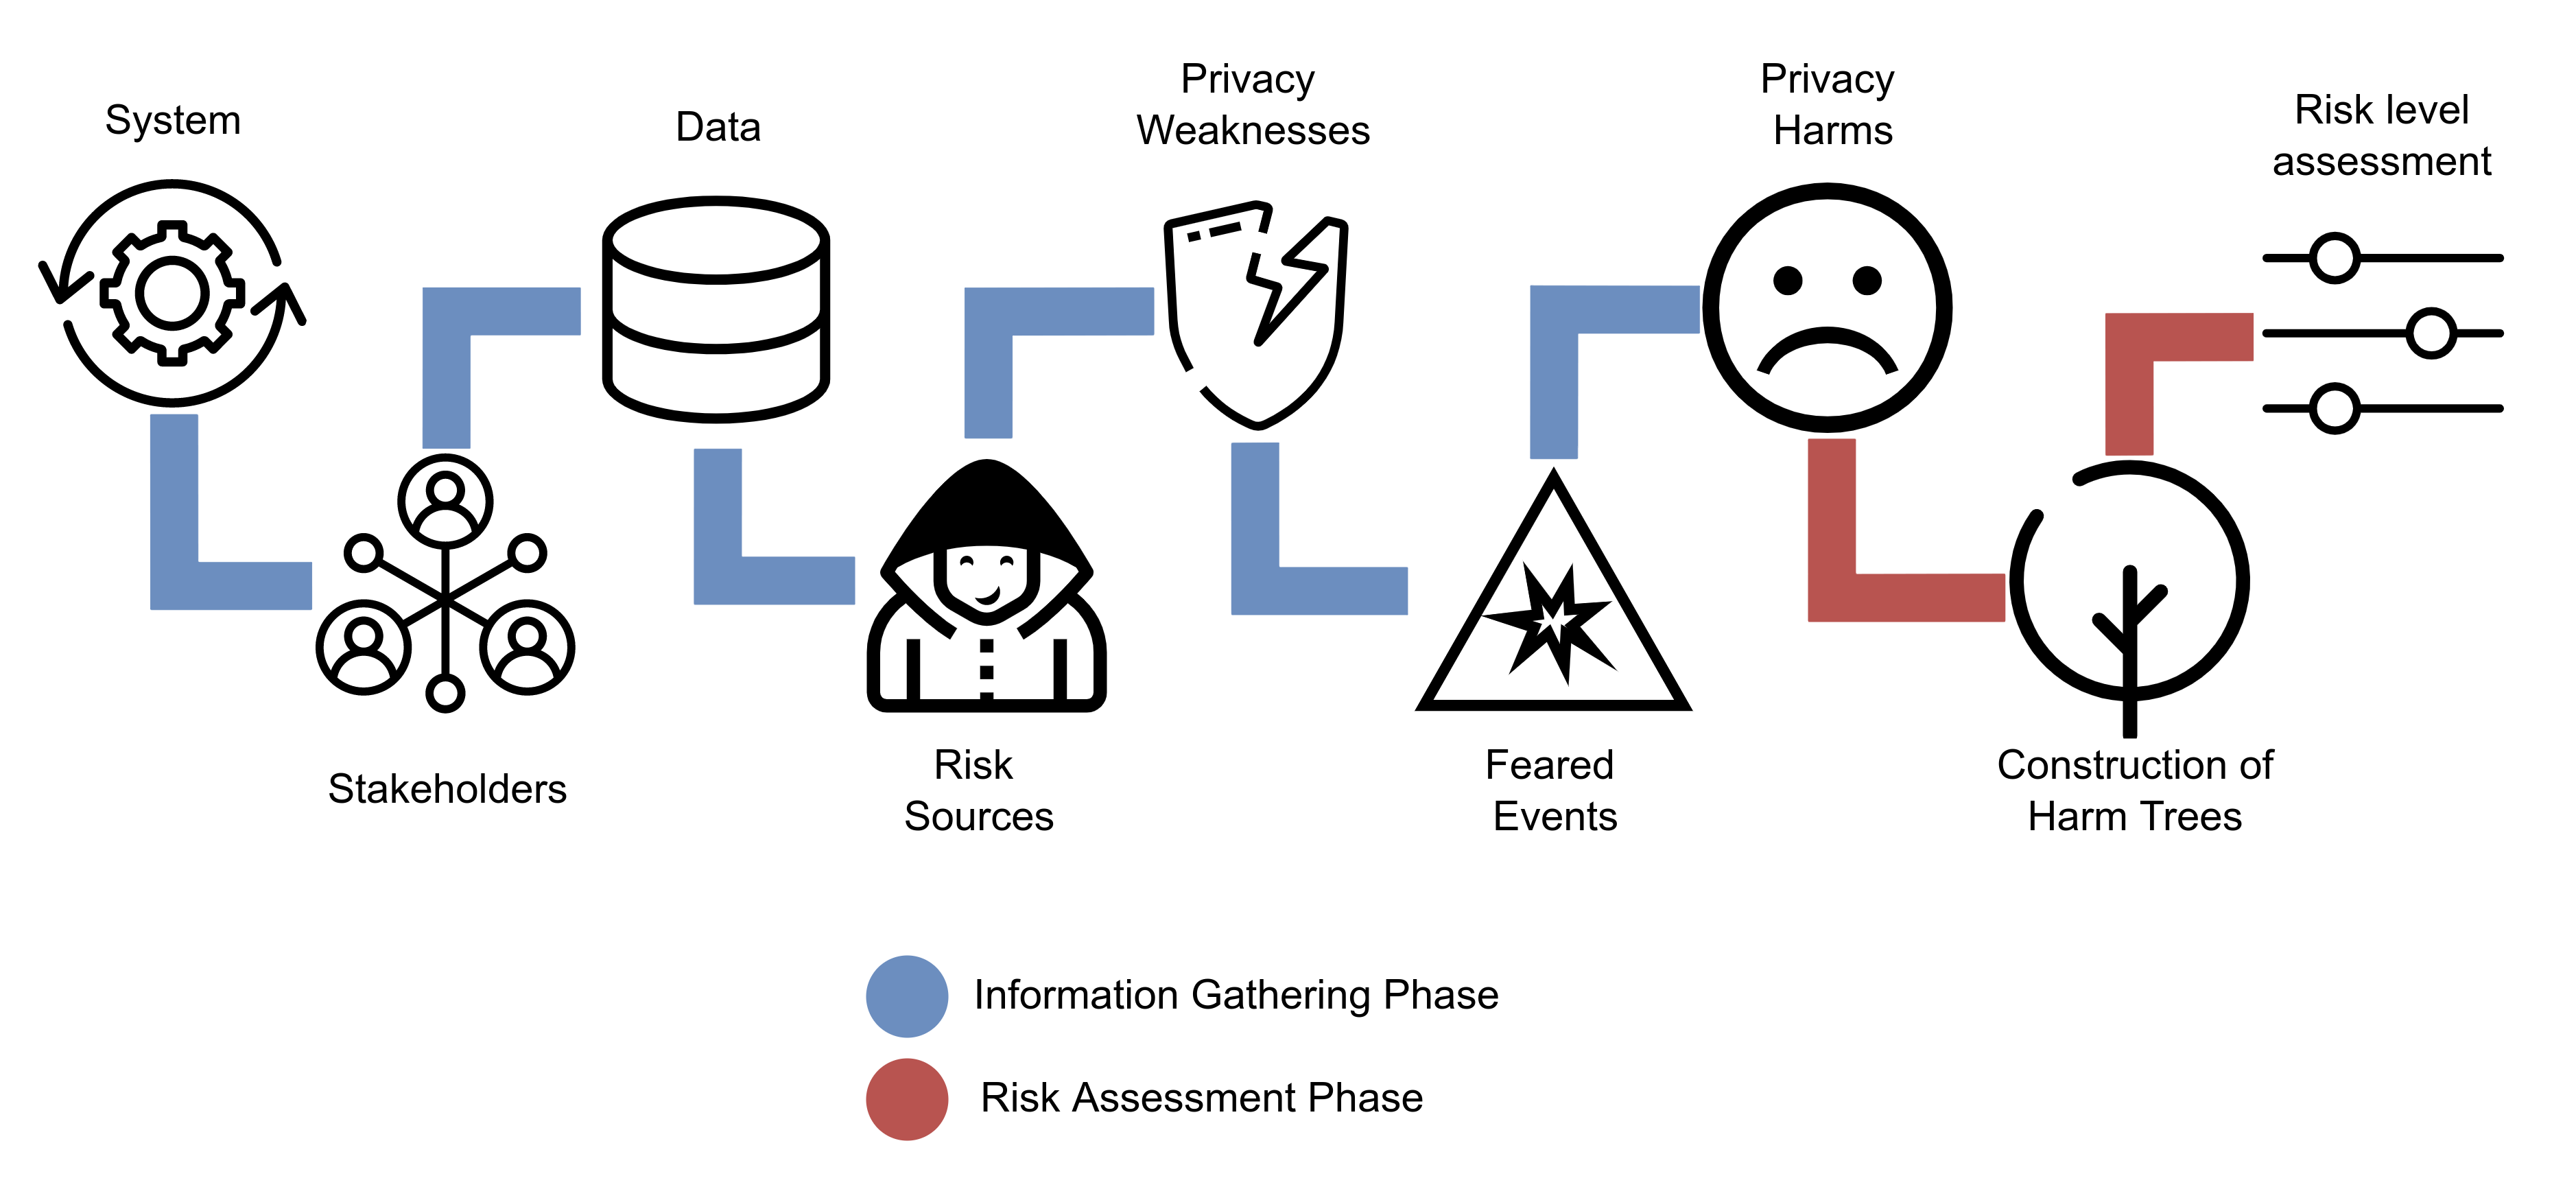
\includegraphics[width=\textwidth]{pictures/priam_model.png}
  \caption{}{The PRIAM methodology process\footnotemark.}
  \label{fig:priam}
\end{figure}

%% Hacky, but works (in order to bypass footnote restrictions in image caption)
\footnotetext{All icons used are from https://thenounproject.com}

The PRIAM methodology process (see Figure \ref{fig:priam}) is split into two
phases, the first of which being the \textit{Information Gathering Phase}. The
main objective in this phase is to gather the relevant information needed in
order to accurately carry out the risk assessment activities in the \textit{Risk
Assessment Phase}.

\subsection{Information Gathering Phase}
As the foundation for the upcoming risk assessment, it is essential that the
information collected in this phase is complete. To reduce the likelihood of an
analyst missing aspects that may have an impact on privacy risks, the framework
defines seven \textit{components}. These components, namely the \textit{system},
\textit{stakeholders}, \textit{data}, \textit{risk sources}, \textit{privacy
weaknesses}, \textit{feared events} and \textit{privacy harms} are each
associated with a set of \textit{categories} and \textit{attributes}. A category
is essentially a list of elements relevant to a specific component, while
attributes describes the characteristics of a component that may affect privacy
risks\cite{de2016priam}.

\begin{figure}[hbt!]
  \centering
  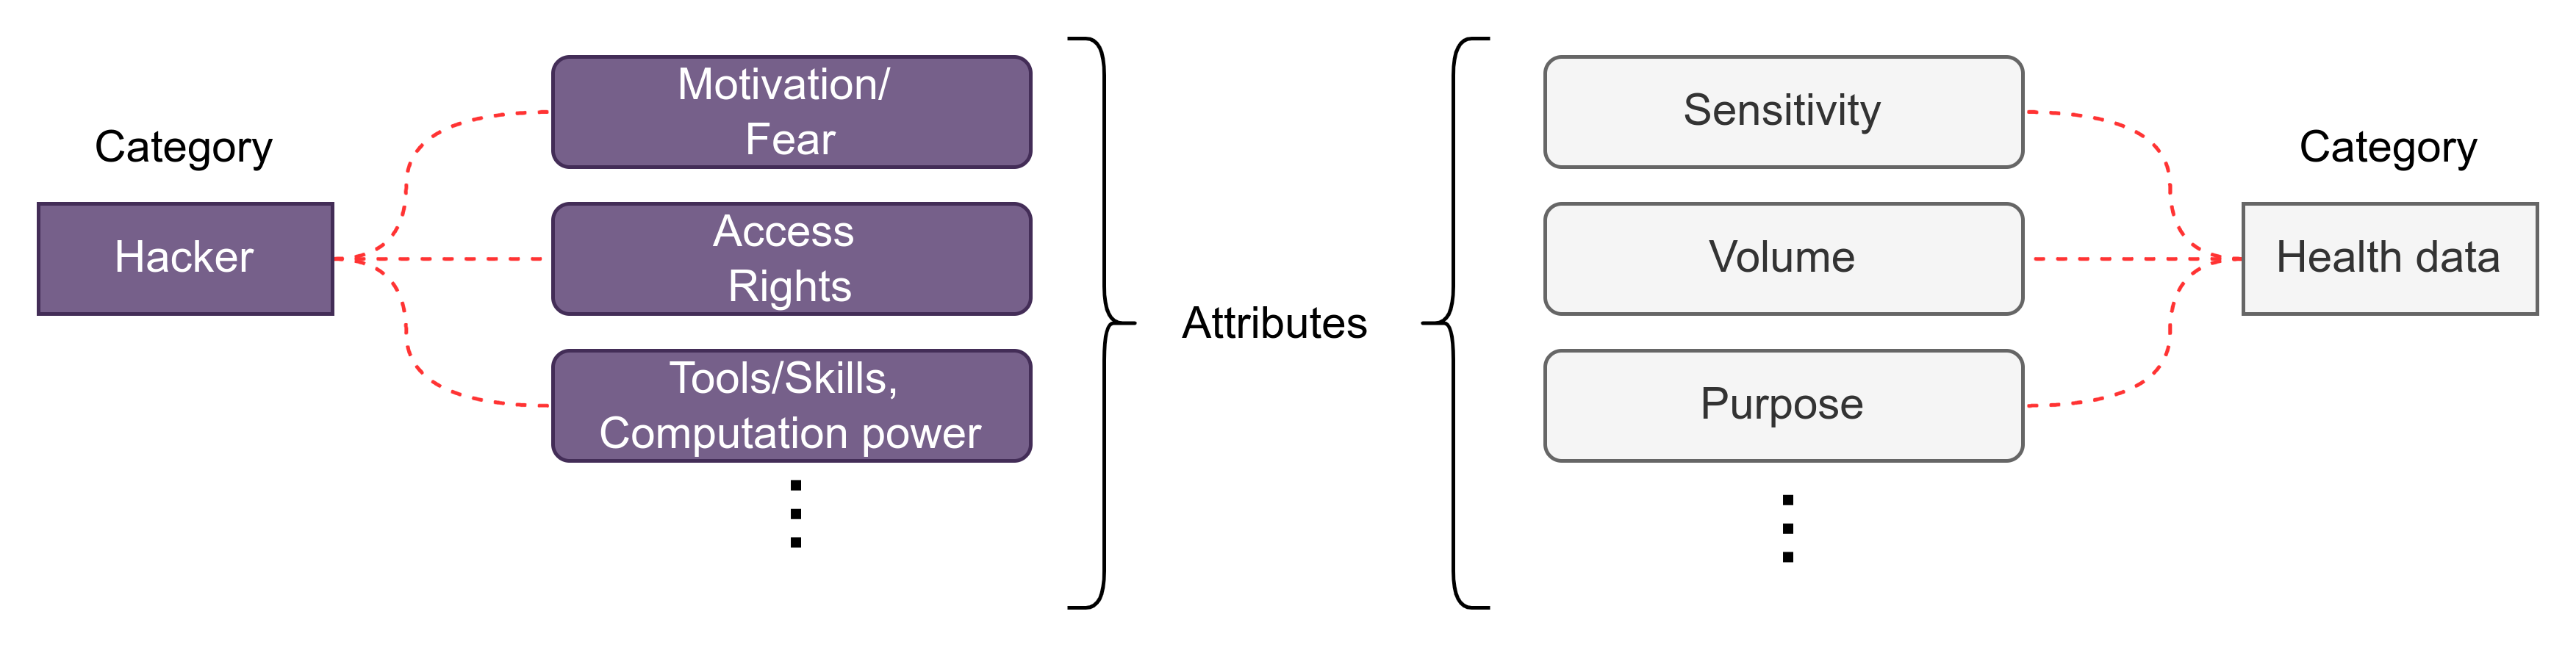
\includegraphics[width=\textwidth]{pictures/cat_att.png}
  \caption{}{Categories with their associated attributes.}
  \label{fig:cat_att}
\end{figure}

In Figure \ref{fig:cat_att} an example is given to illustrate this concept
further. The potential or capability of the risk source, in this case the
\textit{Hacker} (which is the category), would be determined by the assigned
values of its attributes. Similarly for \textit{Health data}, which is a
category of the \textit{data} component, the attributes could indicate a
potential privacy weakness. The categories and their corresponding attributes
are however not only used for indicative purposes, but for constructing harm
trees and calculating risk levels in the next phase.

\subsection{Risk Assessment Phase}
With basis in the information collected in the \textit{Information Gathering
Phase}, we are set to perform the risk assessment. In order to calculate the
risk levels associated with a given scenario, so-called \textit{harm trees} are
constructed.

\begin{figure}[hbt!]
  \centering
  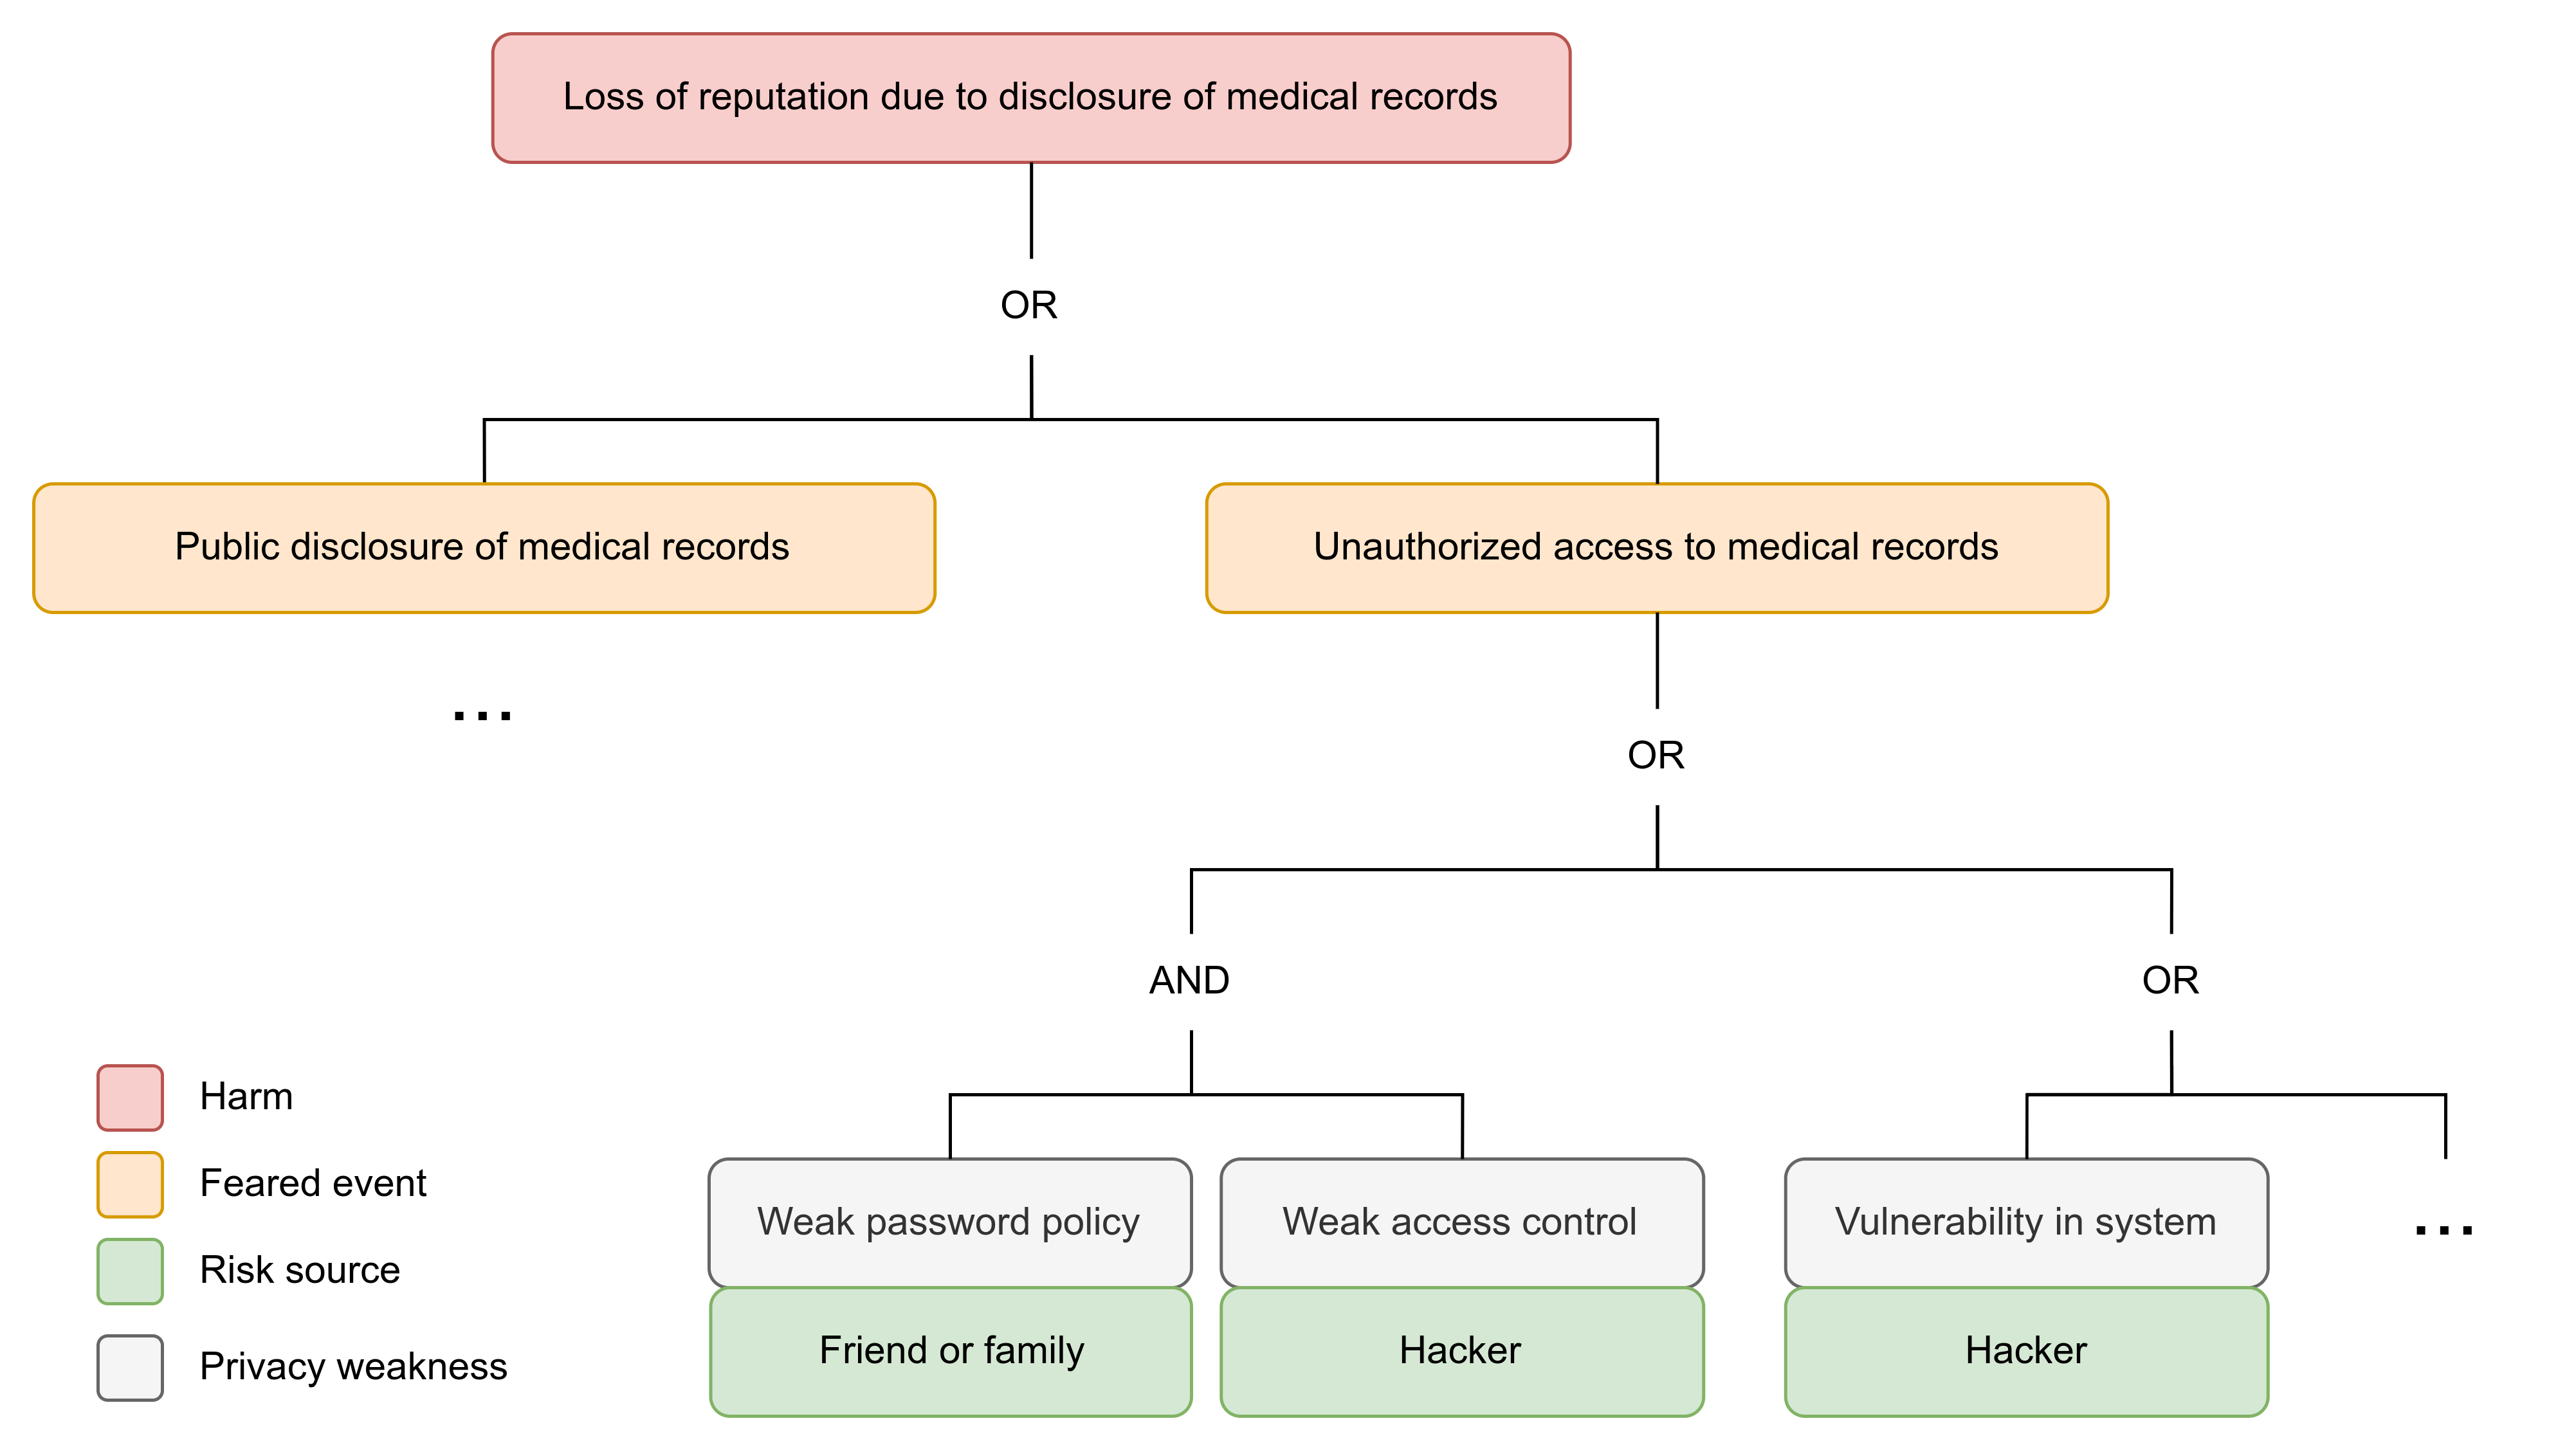
\includegraphics[width=0.7\textwidth]{pictures/harm_tree_ex.png}
  \caption{}{Harm tree example.}
  \label{fig:harm_tree_ex}
\end{figure}

Harm trees (see Figure \ref{fig:harm_tree_ex}), similarily to attack trees
commonly used in computer security\cite{de2016priam}, are used to describe the
relationship between a privacy weakness, a feared event and a harm (REF all
these). The root node of such a tree will denote a harm, with branches leading
to feared events that may lead to the harm in question. The leaf nodes denote
privacy weaknesses and are represented by a pair consisting of the most relevant
risk source coupled with a privacy weakness. In order to specify whether
multiple events are required for an event to take place, the keywords
\textbf{AND} and \textbf{OR} are used as decorators on the connecting paths
between the nodes.
